\newlecture

\setcounter{chapter}{12}
\setcounter{section}{2}

%\def\textbookchapter{Chapter 12: Vector Calculus}
\def\coursetopicnumber{IV}
\def\topic{Using Parametrizations to Calculate Line Integrals} % this is the printed title
\def\shorttopic{Line integral computation} % short topic
\def\textbookname{Active Calculus} % this is the corresponding textbook
\def\shorttextbookname{AC} % this is the short name for the book
\def\textbooksection{12.3} % corresponding textbook section
\def\textbooksectionurl{https://activecalculus.org/vector/S_Vector_ParamLineIntegrals.html} % URL for textbook section
\def\handoutday{} % this is the printed date

%%%%%%%%% DOCUMENT CONTENT STARTS BELOW

\thispagestyle{plain}
\topstuff
\section{\topic{} \booklink{}}
\label{sec:compute-line-integral}
\subsection{Formula to compute a line integral}
\begin{defn}[Line integral of a vector field over a path]
    Let $\vec{F}$ be a vector field, and let $C$ be a smooth path given by the parametrization $\vec{r}(t)$ for $t$ in $[a,b]$. 
    The \emph{line integral} of the vector field $\vec{F}$ over $C$ is denoted
    \[
        \int\limits_C \vec{F}\dotp \dvr.
    \]
\end{defn}

If $C$ is parametrized by $\vec{r}=\vec{r}(t)$ for $t$ in $[a,b]$, then we have $\dvr=\vec{r}\,'(t)\,\dt$. Thus, we evaluate the line integral by writing 
\medskip

\[
    \int\limits_C\vec{F}\dotp\dvr
    = \phantom{\int\limits_a^b \vec{F} \dotp \vec{r}'(t)\dt.}\hspace{1in}
\]

\medskip 

Finally, recall that if $\vec{r}(t)=\langle x(t),\, y(t)\rangle$, then $\vec{r}\,'(t)=\langle x'(t),\, y'(t)\rangle$. The resulting integral has just one variable ($t$). We can evaluate it using integration methods from Calculus II.

To evaluate the line integral of a 3D vector field over a path in space, we follow the same general method.

%The same result holds if $\vec{r}(t)=\langle x(t),\, y(t),\, z(t)\rangle$.

%The definition of a line integral of a 3D vector field over a path in space is identical, except in that case we have $\vec{r}(t)=\langle x(t),\, y(t),\, z(t)\rangle$, and therefore $\dvr=\langle \dx,\, \dy,\, \dz\rangle$.


\vfill 

\begin{framed}
    {\textbf{Process to evaluate the line integral of $\vec{F}(x,y)$ over a path $C$ in the plane}}
    \begin{enumerate}
        \item Determine a parametrization $\vec{r}(t)=\langle x(t),\, y(t)\rangle$ for the path $C$ along with an interval $[a,b]$ of $t$-values.
        \item Determine $\vec{F}(\vec{r}(t))$, replacing the $x$ and $y$ in the formula for $\vec{F}(x,y)$ with the $x(t)$ and $y(t)$ from the parametrization.
        \item Determine $\vec{r}\,'(t)=\langle x'(t),\, y'(t)\rangle$ by taking the derivative of each component.
        \item Compute the dot product $\vec{F}(\vec{r}(t))\dotp\vec{r}\,'(t)$. The result is a scalar-valued function of $t$.
        \item The line integral is then
        \[\int\limits_C \vec{F}\dotp\dvr = \int\limits_a^b \vec{F}(\vec{r}(t))\dotp\vec{r}\,'(t)\dt.\]
        \item Evaluate the integral using integration techniques from Calculus II.
    \end{enumerate}
    Note: To evaluate the line integral of $\vec{F}(x,y,z)$ over a path $C$ in space, the process is the same.
\end{framed}
\pagebreak 

\subsection{Some examples}
\begin{ex}
    Let $\vec{F}(x,y)=\langle y,-x\rangle$. Let $C_1$ be the curve given by $\vec{r}(t)=\langle \cos(t),\sin(t)\rangle$ for $0\le t\le \pi$. Let $C_2$ be the path along the $x$-axis from the point $(1,0)$ to the point $(-1,0)$. A sketch of $\vec{F}$ appears below.
    \begin{enumerate}
        \item Based on the picture, will the line integral of $\vec{F}$ over $C_1$ be positive, negative, or zero?
        \item Based on the picture, will the line integral of $\vec{F}$ over $C_2$ be positive, negative, or zero?
        \item Compute both line integrals.
    \end{enumerate}
    \mbox{}\hfill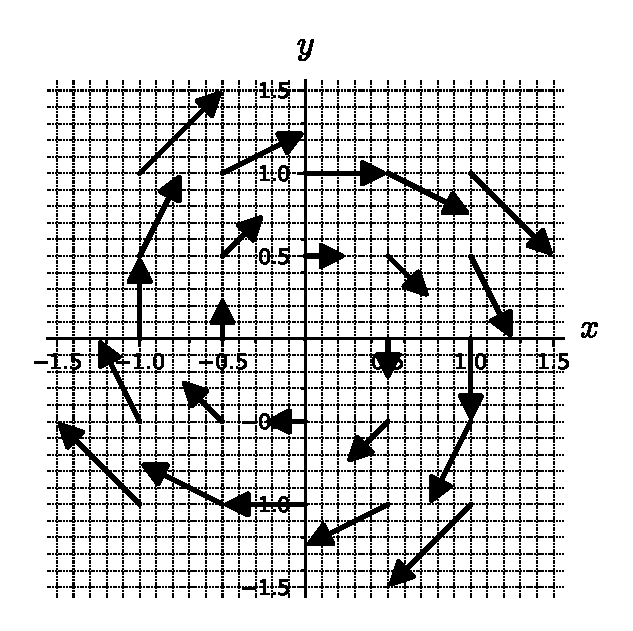
\includegraphics[scale=.8]{images/cw-circulating-vf.eps}\label{img:sage-vector-field-4}
\end{ex}
\pagebreak 
\begin{ex}
    Let $\vec{F}(x,y,z)=\langle xy,yz,xz\rangle$ and $C$ be parametrized by $\vec{r}(t)=\langle t,t^2,t^3\rangle$. 
    \\ 
    Compute the line integral of $\vec{F}$ over $C$ for $0\le t\le 1$.
\end{ex}

\vfill 

\pagebreak 

\begin{ex}
    Let $\vec{F}(x,y)=\langle 5-2x,\,\sin(y)\rangle$. Let $C$ be the path that starts at the origin, goes to the point $(2,4)$ along the graph of $y=x^2$, and then goes to the point $(2,0)$ along a straight line. Compute the line integral of $\vec{F}$ over $C$.
\end{ex}

\vfill

\pagebreak 

\subsection{Alternative line integral notation}
For a 2D vector field $\vec{F}(x,y)$ and a path $C$ parametrized by $\vec{r}(t)=\langle x(t),y(t)\rangle$ for $a\le t\le b$, we know from the start of this section that the line integral of $\vec{F}$ over $C$ is written 
\[
    \int\limits_C \vec{F}\dotp\dvr
    = \int\limits_a^b \vec{F}(\vec{r}(t))\dotp\vec{r}\,'(t)\dt.
\]

For the 2D vector field $\vec{F}$, we have 
\[
    \vec{F}(x,y)=\langle F_1(x,y),\, F_2(x,y)\rangle
\]
for some scalar-valued functions $F_1(x,y)$ and $F_2(x,y)$. Since $\vec{r}=\langle x,y\rangle$, we also have 
\[
    \dvr = \langle \dx,\, \dy\rangle.
\]

\begin{ex} 
    Compute $\vec{F}\dotp\dvr$.
    %\[
    %    \vec{F}\dotp\dvr = \langle F_1(x,y),\, F_2(x,y)\rangle \dotp \langle \dx,\, \dy\rangle = \phantom{F_1(x,y)\dx + F_2(x,y)\dy.}
    %\]
\end{ex}

\vfill

We may alternatively write the line integral as 
\[
    \int\limits_C \vec{F}\dotp\dvr
    = \phantom{\int\limits_C F_1(x,y)\dx + F_2(x,y)\dy.}
\]

\begin{defn}[Differential form]
    For scalar-valued functions $F_1(x,y)$ and $F_2(x,y)$, the quantity 
    \[F_1(x,y)\dx + F_2(x,y)\dy\]
    is called a \emph{differential form}.
\end{defn}

All of the above holds if $\vec{F}$ is a 3D vector field as well:

\vfill
\begin{ex}
    For some path $C$, suppose we have the line integral 
    \[
        \int\limits_C (3x+y)\dx + 2xy\dy.
    \]
    For what vector field $\vec{F}$ is this line integral equal to the line integral $\displaystyle\int\limits_C \vec{F}\dotp\dvr$?
\end{ex}

\vspace{.5in}

%\item Let $\vec{F}(\langle x,y,z\rangle)=\langle z,x,y\rangle$ and let $C$ be parametrized by $\vec{r}(t)=\langle \cos(t),\sin(t),t\rangle$ for $0\le t\le 2\pi$. Compute the line integral of $\vec{F}$ over $C$.

